%Formatvorgabe tobii ist toll beim Kellerpumpen
\documentclass[12pt,a4paper,oneside,bibliography=totocnumbered]{scrartcl}
\usepackage[ngerman]{babel}
\usepackage[utf8]{inputenc}
\usepackage[a4paper,left=4cm,right=2cm,top=3cm,bottom=2cm]{geometry}
\linespread{1.25}
\usepackage{fancyhdr}
\pagestyle{fancy}
\lhead{}
\rhead{\thepage}
\cfoot{}



%Hier sind die Daten der Seminararbeit
\newcommand{\MyAuthor}{Tobias Wäschle (285524) \& René Spieker}
\newcommand{\MyTitel}{SAP ERP - Rechnungswesen (FI, CO)}
\newcommand{\MyFirma}{Deutsche Telekom AG}
%\newcommand{\MyMatrikelNummer}{285524}
\newcommand{\MyBetreuer}{Dr.-Ing. Peter Steininger}
\newcommand{\MyKurs}{ERP-Systeme}
\newcommand{\MySemester}{4. Fachsemester}
\newcommand{\MyStudiengang}{Wirtschaftsinformatik}
\newcommand{\MyOrt}{Bonn}
\newcommand{\MyDatum}{\today}


\usepackage{floatflt}
\usepackage{graphicx}
\usepackage{caption}
%Abkürzungsverzeichnis z.B. etc.\abk{etc.}{et cetera}
\usepackage{nomencl}
\usepackage{paralist}
\usepackage{mathptmx}
\usepackage{natbib}
\usepackage[hidelinks,
			pdfauthor={\MyAuthor},
			pdftitle={\MyTitel},
			pdfproducer={pdfLaTeX with hyperref},
			pdfcreator={pdfLaTeX}]{hyperref}

\author{\MyAuthor}
\title{\MyTitel}
\date{\MyDatum}

% Befehl für Abkürzungen umbenennen in abk
\let\abk\nomenclature
% Deutsche Überschrift
 \renewcommand{\nomname}{}
 % Punkte zw. Abkürzung und Erklärung
 \setlength{\nomlabelwidth}{.35\hsize}
 \renewcommand{\nomlabel}[1]{#1 \dotfill}
 % Zeilenabstände verkleinern
 \setlength{\nomitemsep}{-\parsep} 
 \makenomenclature

\makeindex



\begin{document}

%Titelseite
\begin{titlepage}
\raggedleft

\centering
\vfill
{\bfseries\Huge Seminararbeit}\\
\vfill
Titel der Seminararbeit\\[2ex]
{\bfseries\Large "`\MyTitel{}"'}\\[1ex]
{\bfseries\small -- \MySemester{} --}\\
\vfill
Verfasser: \MyAuthor{}\\
\vfill
\raggedright
\small
\MyOrt, den \MyDatum\\[2cm]
\begin{tabbing}
%Matrikelnummer: \= \MyMatrikelNummer{}\\
Studiengang: \= \MyStudiengang{}\\
Kurs: \> \MyKurs{}\\
Betreuer:  \> \MyBetreuer{}\\
\end{tabbing}
\end{titlepage}
\newpage
 
\renewcommand{\thesection}{\Roman{section}}  % I, II, III, IV
\pagenumbering{Roman}

%Weitere Seiten vor dem Hauptteil
%Sperrvermerk
\thispagestyle{empty}
\section*{Sperrvermerk}
Die vorliegende Seminararbeit mit dem Titel ``\MyTitel{}'' enthält unternehmensinterne Daten der Firma \MyFirma{} daher ist sie nur zur Vorlage bei der FOM sowie den Begutachtern der Arbeit bestimmt. Für die Öffentlichkeit und dritte Personen darf sie nicht zugänglich sein.
\\[3cm]
\begin{flushright}
\line(1,0){100} \hfill \line(1,0){150}\\
(Ort, Datum) \hfill \textbf{René Spieker}\\[1.5cm]
\line(1,0){100} \hfill \line(1,0){150}\\
(Ort, Datum) \hfill \textbf{Tobias Wäschle}\\
\end{flushright}

%Inhaltsverzeichnis
\newpage
%\thispagestyle{empty}
\tableofcontents
\clearpage

%Hauptteil
\setcounter{section}{0}
\renewcommand{\thesection}{\arabic{section}} % 1, 2, 3, 4 ...
\pagenumbering{arabic}

\section{Einleitung}
\subsection{Einführung und Relevanz des Themas}
%Viele Unternehmen sehen sich neuen Aufgabenstellungen gegen{\"u}ber. Ursache sind die Internationalisierung, die h{\"a}ufigen Produktwechsel und der Zwang zu permanenter\\Veränderung. Der Anteil der Routineaufgaben nimmt stetig ab, w{\"a}hrend andererseits neuartige und komplexer werdende Aufgaben anstehen\footnote{Vgl. \cite{Fiedler2008}, S.~1}.
%Die Durchführung dieser Aufgaben wird in der Unternehmenspraxis zunehmend in Form von Projekten vollzogen.
%Dass komplexe, neuartige und interdisziplinäre Projekte nicht intuitiv ausgewählt und zum Ziel geführt werden können, dürfte heute jedem Unternehmer klar sein.
%
%In diesem Zusammenhang treten facettenreiche und h{\"o}chst unterschiedliche Problemfelder auf, denen von Seiten der Unternehmenspraxis wie auch der Betriebswirtschaftslehre begegnet werden muss. Um eine geeignete Projektauswahl und Implementierung der Unternehmensstrategien in diese Projekte zu gewährleisten, muss die Unternehmensf{\"u}hrung und die Projektleitung durch eine sinnvolle und methodisch gepr{\"a}gte Planung und Kontrolle der Projekte eines Unternehmens unterst{\"u}tzt werden\footnote{Vgl. \cite{Kunz2007}, S.~1} \footnote{Vgl. \cite{Urli&Terrien2010}}.

\subsection{Zielsetzung und Abgrenzung}
%Diese Arbeit beschäftigt sich mit theorieorientierten Ausprägungen und Beschreibungen des Projektcontrollings. Das Thema wird in sinnvollen Aufgabenbereichen strukturiert und näher analysiert. Es werden die Grundlagen des Projektmanagement vorausgesetzt und deshalb auf eine detaillierte Beschreibung der Methoden und Techniken der Organisation, Planung und Durchführung von Projektportfolios oder Projekten verzichtet.

\subsection{Vorgehen}
%Die Abbildung \ref{abb1} auf Seite \pageref{abb1} zeigt eine schematische Darstellung zum Aufbau der Arbeit.
%\begin{figure}[htbp]
%\begin{center}
%%\begin{floatingfigure}[r]{0.7\textwidth}
%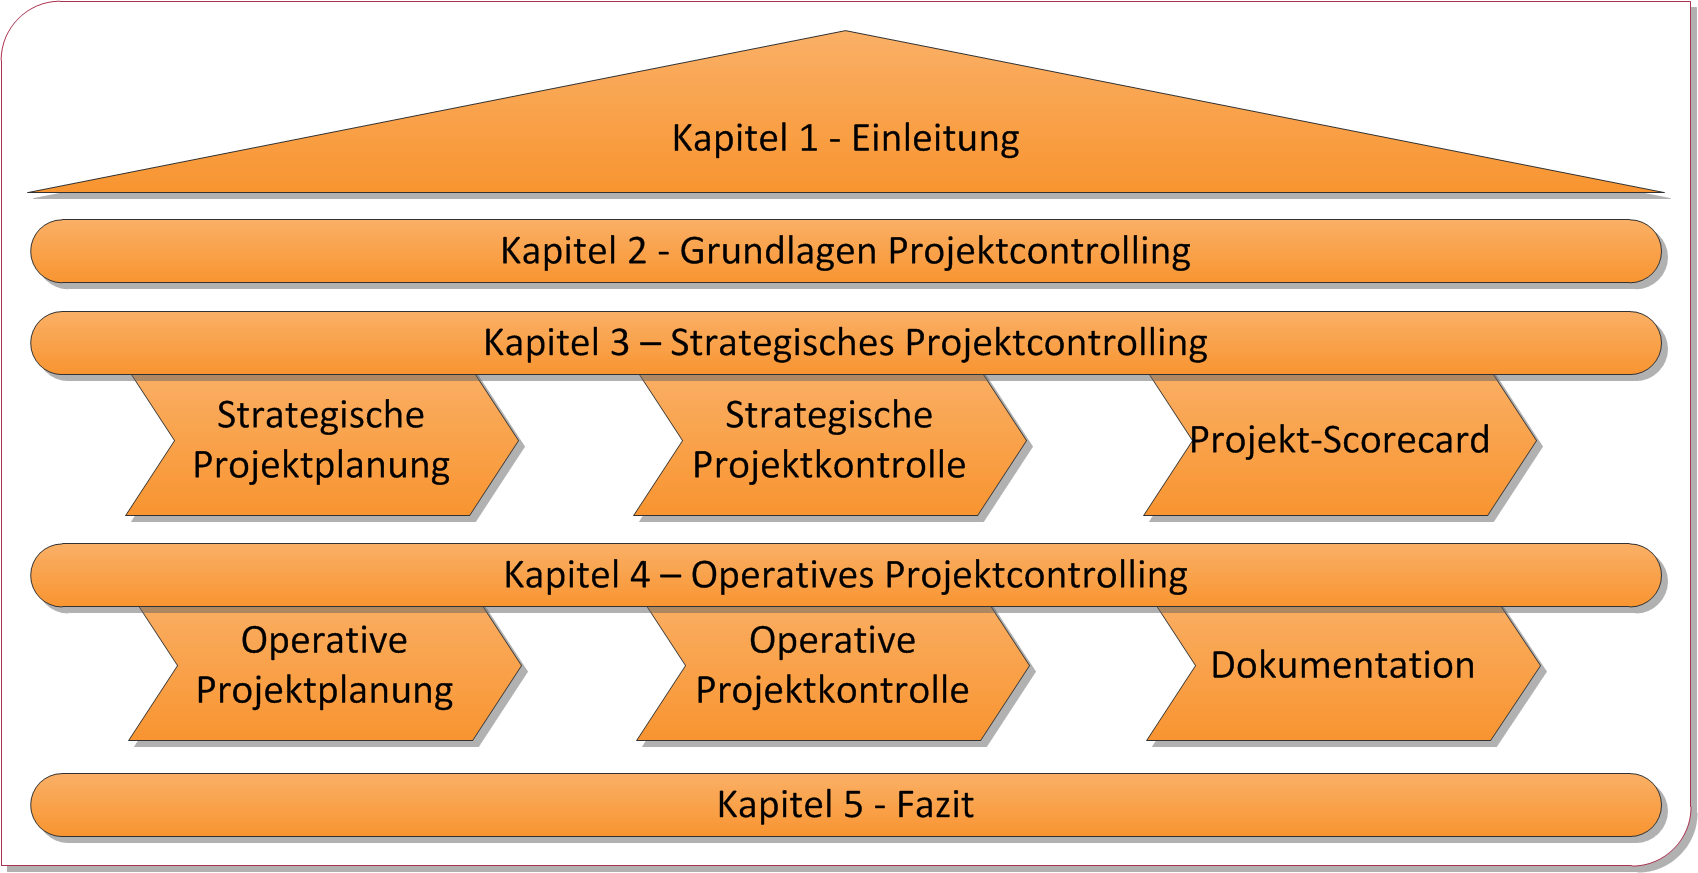
\includegraphics[width=0.8\textwidth]{Images/aufbau.png}
%\caption[Aufbau dieser Arbeit]{Aufbau dieser Arbeit}
%\label{abb1}
%\end{center}
%\end{figure}
%%\end{floatingfigure}
%\begin{compactitem}
%\item Kapitel 1 führt an das betrachtete Thema heran und definiert die Ziele dieser Arbeit.
%\item Kapitel 2 gibt einen Überblick über Projektcontrolling im Projektmanagement. Angesprochen werden die Ausprägungen, sowie die Aufgaben und Ziele des Projektcontrollings.
%\item Kapitel 3 behandelt das Projektcontrolling aus strategischer Sicht. Es wird die Auswahl und Priorisierung von Projekten in einem Projektportfolio erklärt, aber auch um den Einsatz der Project Scorecard für die Projektauswahl und Projektsteuerung.
%\item Kapitel 4 bildet den Schwerpunkt der Arbeit. Es beschreibt das operative Projektcontrolling und orientiert sich an den Lebenszyklusphasen eines Projektes. Die Sicht auf die Planung wird um die Aspekte der Steuerung und Kontrolle ergänzt.
%\item Kapitel 5 [...]tbd
%\end{compactitem}



\section{Grundlagen Rechnungswesen}
\subsection{externes Rechnungswesen}\label{ssec:externesRechnungswesen}
\abk{Financial Accounting}{externes Rechnungswesen, Finanzwesen -- FI}

hier kopieren\footnote{\cite{SAPFI2001}}



\subsection{internes Rechnungswesen}
\label{ssec:internesRechnungswesen}
\abk{Management Accounting}{internes Rechnungswesen, Controlling -- CO}
Der Bereich des betrieblichen Rechnungswesens übernimmt eine besondere Dokumentations- und Kontrollfunktion in einer Wirtschaftsunternehmung.
Die externen orientierten Aufgaben sind meist durch gesetzliche Vorgaben eingeschränkt und dienen der Rechenschaftslegung gegenüber Gesellschaftern, Gläubigern, der Öffentlichkeit und dem Staat (Vgl. s. Kapitel \ref{ssec:externesRechnungswesen} auf S. \pageref{ssec:externesRechnungswesen}).
Die intern orientierten Aufgaben unterliegen hingegen keinerlei sachfremden und gesetzlichen Vorgaben und können so den individuellen Ansprüchen des Managements angepasst werden. Das interne Rechnungswesen (Betriebsbuchhaltung oder Management Accounting) dient der mengen- und wertmäßig Erfassung sowie\\ Überwachung aller in einem Unternehmen auftretenden Geld- und Leistungsströme. Es ist typischerweise kurzfristig ausgerichtet und weist kürzere Abrechnungszeiträume als das Geschäftsjahr des externen Rechnungswesens auf\footnote{Vgl. \cite{Wohe2000}, S. 853}\footnote{Vgl. \cite{Schierenbeck2008}, S. 799}.
Die Tabelle \ref{abb1} (S. \pageref{abb1}) stellt die wichtigsten Unterscheidungsmerkmale zwischen dem internen und dem externen Rechnungswesen dar.\\
\begin{table}[htbp]
\begin{center}
\caption[Vergleich externes- und internes Rechnungswesen]{Vergleich externes- und internes Rechnungswesen}
\includegraphics[width=1\textwidth]{Images/VergleichIntExt.png}
\label{abb1}
{\footnotesize In Anlehnung an: \cite{Lojewski2001}, S. 6}
\end{center}
\end{table} 

\noindent Es ergeben sich 3 Hauptaufgaben im internen Rechnungswesen\footnote{Vgl. ebd., S. 799}:
\begin{compactitem}
\item[1] Die Ermittlung des kurzfristigen Betriebserfolgs
\item[2] Kontrolle der Wirtschaftlichkeit und Budgetierung
\item[3] Rechnerische Fundierung unternehmenspolitischer Entscheidungen
\end{compactitem}

\subsubsection{Ermittlung des kurzfristigen Betriebserfolgs}
Zur Erfüllung der genannten Hauptaufgaben der internen Unternehmungsrechnung kommen die Systeme der Kosten- und Leistungsrechnung zum Einsatz\footnote{Vgl. \cite{Schierenbeck2008}, S.~800}. Nach Jörg Wöltje besteht das interne Rechnungswesen aus der Kostenrechnung, der Leistungsrechnung und der Erfolgsrechnung. Die Kostenrechnung dokumentiert die Verbrauchsseite, also die entstandenen Kosten des Produktionsprozesses. Die Leistungsrechnung dokumentiert die Entstehungsseite, also die erzielten Erlöse des Produktionsprozesses. Stellt man Verbrauchs- und Entstehungsseite gegenüber, spricht man von einer Erfolgsrechnung. Die kalkulatorische Erfolgsrechnung als Hauptbestandteil des internen Rechnungswesens wird für einzelne Produkte, Produktgruppen oder Unternehmensbereiche erstellt und soll für kurze Abrechnungszeiträume den Betriebserfolg als Saldo der bewerteten Periodenleistungen und der Periodenkosten ermitteln\footnote{Vgl. \cite{Woltje2008}, S.~179}.
Kernstück ist dabei die Kostenrechnung, die bei entsprechender Ausgestaltung den Prozess der Kostenentstehung schrittweise verfolgt und eine rechnerische Aufgliederung des Kostengefüges 
\begin{compactitem}
\item nach Kostenarten (Welche Kosten fallen an?), 
\item nach Kostenstellen (Wo fallen welche Kosten an?) und 
\item nach Kostenträgern (Wofür, d.h. für welche Leistungen fallen Kosten an?)
\end{compactitem} ermöglicht\footnote{Vgl. \cite{Schierenbeck2008}, S.~799}\footnote{Vgl. \cite{Ossadnik2008}, S~52 ff.}.


\subsubsection{Kontrolle der Wirtschaftlichkeit und Budgetierung}
Wie wirtschaftlich wird in den Kostenstellen gearbeitet?
Aufgrund ihrer internen Ausrichtung fällt der kalkulatorischen Erfolgsrechnung die Aufgabe zu, den Ablauf der Unternehmungsprozesse zu überwachen. Klein sieht in der Kontrolle die Überwachung von Dispositionen untergeordneter Instanzen. Dabei kann Kontrolle definiert werden als die \glqq Durchführung eines Vergleichs zwischen einer zu prüfenden und einer Plangröße\grqq \footnote{Vgl. \cite{Klein1999}, S.~22}.
Dieses Instrument zeigt, welche Produkte am stärksten am Umsatz beteiligt sind. Auch wird klar, welche Produktelemente die höchsten Kosten verursachen und deshalb besonders beachtet werden sollten. So werden Schwachstellen und Unwirtschaftlichkeiten im Leistungserstellungsprozesses erkannt\footnote{Vgl. \cite{Woltje2008}, S.~196 f.}. Mit dem Ziel, vorgegebene Kostendeckungs-, Gewinn- oder Rentabilitätsziele sicher zu stellen, wird die kalkulatorische Erfolgsrechnung auch für die Budgetierung von Kosten und Erlösen eingesetzt\footnote{Vgl. \cite{Schierenbeck2008}, S.~800}.

\subsubsection{Rechnerische Fundierung unternehmenspolitischer Entscheidungen}
Der internen Unternehmungsrechnung kommt hier die Aufgabe zu, das Zahlenmaterial für Entscheidungsrechnungen im Sinne von Planungsrechnungen zu liefern. Diese Funktion dient sowohl der Entscheidungsfindung als auch dem Entscheidungsvollzug\footnote{Vgl. \cite{Klein1999}, S.~22}\footnote{Vgl. \cite{Schierenbeck2008}, S.~800}.\\
Zu den Hauptaufgaben zählen hier in erster Linie\footnote{Vgl. ebd., S.~800}: 
\begin{compactitem}
\item die Kalkulation von Preisen und Preisuntergrenzen, 
\item die Planung des Mitteleinsatzes im Marketing, 
\item die Produktions- und Absatzplanung, 
\item die Produktionsdurchführungsplanung, 
\item die Materialbereitstellungsplanung (einschließlich Wahl zwischen Eigenfertigung und Fremdbezug) \\sowie 
\item die Investitions- und Finanzierungsprogrammplanung. 
\end{compactitem} 





%Das Projektcontrolling ist neben der Projektplanung und Führung eine Instanz des Projektmanagements. Auch in anderen Betriebswirtschaftlichen Bereichen ist das Controlling etabliert. In diesem Kapitel wird anhand der allgemeinen Definitionen, der Brückenschlag zwischen Controlling und dem Projektcontrolling aufgezeigt.
%\subsection{Projekt und Projektmanagement}
%\label{ssec:Projekt}
%Um gleich zu Beginn ein einheitliches Verständnis zu schaffen, bedarf es der grundsätzlichen Definition der Begriffe Projekt und Projektmanagement.
%
%Projekte sind heute nicht mehr wegzudenken und in allen Bereichen der Wirtschaft in unterschiedlichsten Ausprägungen zu finden. Gerade neuartige, einmalige oder besonders komplexe Vorhaben lassen sich nicht in bestehenden Linienorganisationen bearbeiten und erfordern meist interdisziplinäre Organisationen. \label{69901Projekt} Die DIN 69901 definiert ein Projekt als ein Vorhaben, das im Wesentlichen gekennzeichnet ist durch:
%\begin{compactitem}
%\item die Einmaligkeit der Bedingungen 
%\item eine projektbezogene Zielvorgabe 
%\item eine zeitliche, finanzielle und personelle Begrenzung 
%\item Abgrenzung gegenüber anderen Projekten 
%\item eine projektspezifische Organisation
%\end{compactitem}
%%\begin{figure}[htbp]
%\begin{floatingfigure}[r]{0.4\textwidth} 
%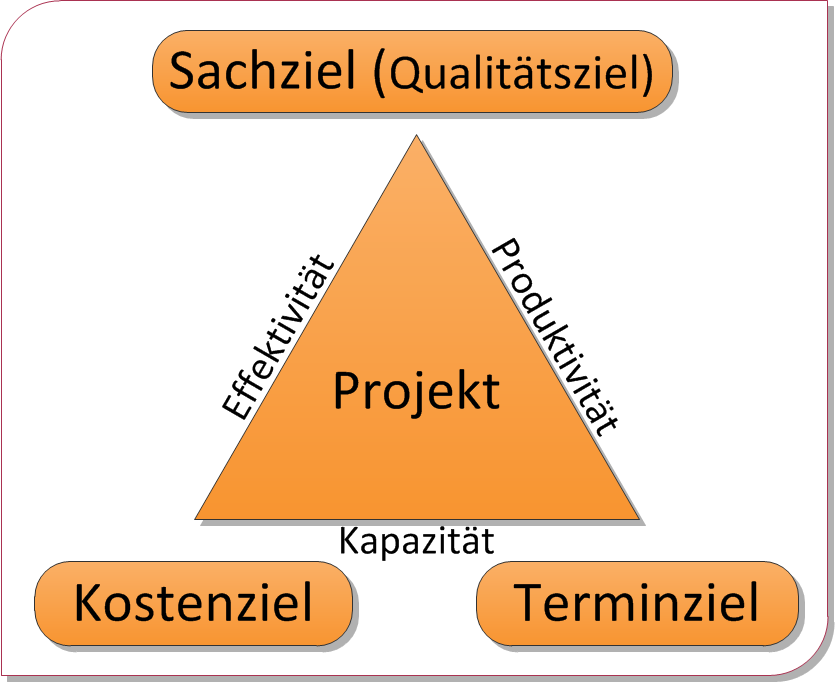
\includegraphics[width=0.4\textwidth]{Images/magischesDreieck.png}
%\begin{center}
%   {\footnotesize In Anlehnung an: \cite{Wischnewski1991}}
%   \caption[Magisches Dreieck]{Magisches Dreieck}\label{abb2}
%\end{center}
%\end{floatingfigure}\noindent
%Es stellt sich die Frage, welche Parameter entscheidend für den Erfolg eines Projektes sind. Aus den oben genannten Merkmalen lassen sich die Parameter Qualität des Ergebnisses (Sachziel), Kosten (Kostenziel) und Dauer (Terminziel) ableiten. Diese Ziele beeinflussen sich gegenseitig und bilden das so genannte „magische“ Dreieck der Projektorganisation (siehe Abbildung \ref{abb2} auf S. \pageref{abb2})\footnote{Vgl. \cite{Wegmann&Winklbauer2006}}
%Typisch für viele Projekte ist, dass man anfangs nicht weiß, ob die angestrebten Ziele überhaupt erreicht werden können. Häufig wird der Zeitrahmen nicht eingehalten, die Kosten werden überschritten, oder man ist nicht in der Lage, die erhoffte Qualität zu erbringen\footnote{Vgl. \cite{Fiedler2008}, S.~3}.
%
%Die Aufgabe des Projektmanagements besteht darin, dafür zu sorgen, dass das Vorhaben unter der Berücksichtigung der Projektziele durchgeführt wird. Das Projektmanagement nimmt dabei bestimmte Funktionen wie etwa Planung, Führung und Controlling wahr\footnote{Vgl. \cite{Bergmann&Garrecht2008}, S.~209}. Nach DIN 69901 versteht man unter dem Begriff  Projektmanagement: \label{69901Projektmgmt}\begin{quote}Projektmanagement ist die Gesamtheit von Führungsaufgaben, -organisation, -techniken und –mitteln für die Abwicklung eines Projekts.\end{quote}\par 
%
%\subsection{Controlling}
%\label{ssec:c}
%Controlling hat sich in den letzten Jahren zu einer festen Institution in den Unternehmen entwickelt. Es gibt kaum ein Unternehmen, das keine eigene Abteilung oder zumindest Angestellte hat, die für das Controlling verantwortlich ist. Der Begriff Controlling ist allerdings sehr weit gefasst. Die Anforderungen in den Unternehmen sind so komplex, dass sich das Controlling dezentralisieren muss, um seine Aufgabe erfüllen zu können. Der Controller kann als ein \glqq Beifahrer\grqq  definiert werden, der den \glqq Fahrer\grqq (Manager) beim Steuern des \glqq Fahrzeugs\grqq \ (Unternehmen) unterstützt. Der Fahrer konzentriert sich auf das Steuern und auf die möglichen Reaktionen. Diese Aktivitäten verlangen seine volle Aufmerksamkeit und er kann keine anderen Tätigkeiten wie etwa Kartenlesen verrichten. Der Beifahrer ist freier als der Fahrer. Er kann daher nützliche Dinge tun, die den Fahrer unterstützen\footnote{Vgl. \cite{Pufahl2006}, S.~11}.\newpage
%\begin{floatingfigure}[r]{0.37\textwidth} 
%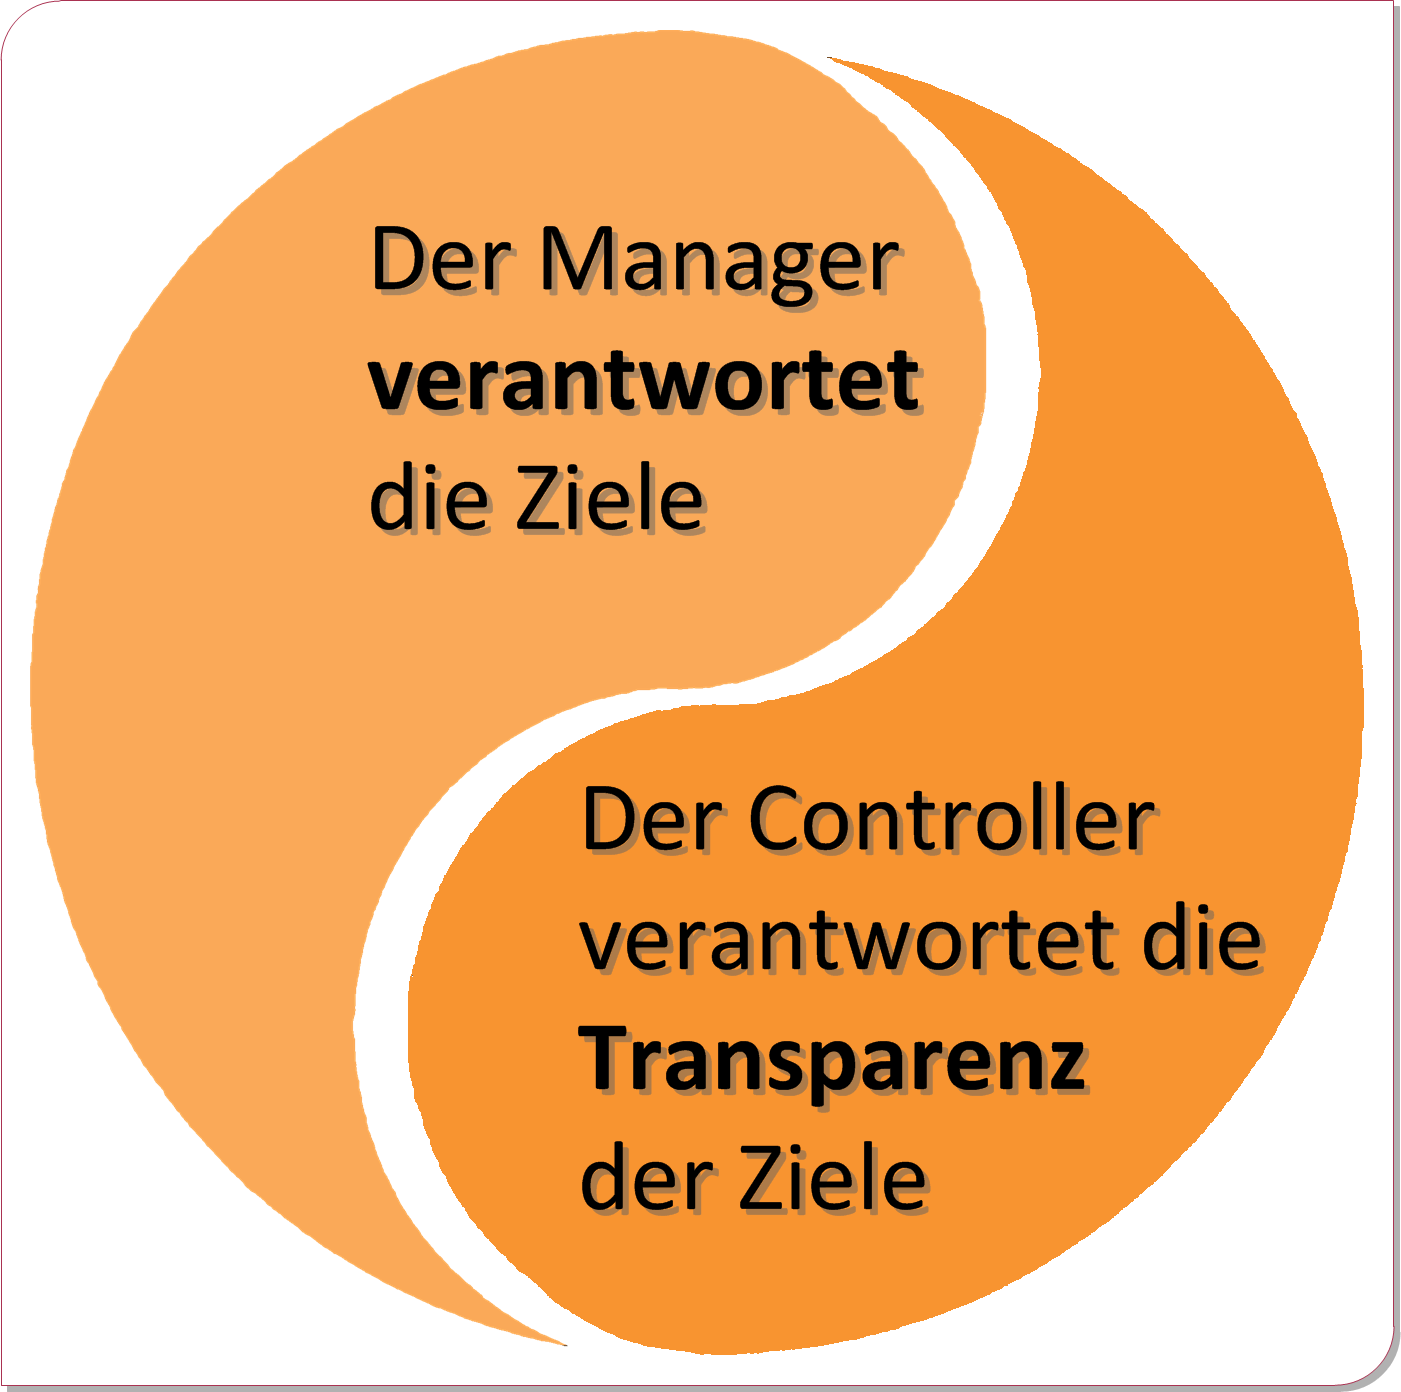
\includegraphics[width=0.37\textwidth]{Images/aufgabenabgrenzungLeiterController.png}
%\begin{center}
%   {\footnotesize In Anlehnung an: \cite{Fiedler2008}, S. 21}
%   \caption[Management vs. Controlling]{Management vs. Controlling}\label{abb4}
%\end{center}
%
%%\end{figure}
%\end{floatingfigure}\noindent
%Controlling hat primär die Aufgabe, zwischen Planung, Kontrolle und Informationsversorgung zu koordinieren (so genannte systemkoppelnde Funktion des Controllings). Die Daten der Planung sind beispielsweise so aufzubereiten, dass eine Kontrolle möglich wird.  Auch innerhalb der Planung und Kontrolle sind Abstimmungen erforderlich. Es muss z. B. der Absatzplan mit dem Produktionsplan und dieser wiederum mit dem Investitionsplan koordiniert werden. Das Controlling stellt auch die Abbildung der strategischen Ziele in der operativen Perspektive sicher. Wichtig ist auch die Gestaltung der genannten Aufgabenbereiche, also die Schaffung von Strukturen und Prozessen. Die systembildende Funktion des Controllings regelt beispielsweise, welche Pläne zu erstellen sind und wie deren Kontrolle funktioniert. Hierzu werden die geeigneten Instrumente und Methoden, sowie die Verantwortlichen festgelegt\footnote{Vgl. \cite{Fiedler2008}, S.~10 f.}.
%\subsection{Projektcontrolling}
%\label{ssec:pc}
%Die DIN 69901 beschreibt das Projektcontrolling als Regelkreis:\begin{quote}Sicherung des Erreichens der Projektziele durch: Soll-Ist-Vergleich, Feststellung der Abweichungen, Bewerten der Konsequenzen und Vorschlagen von Korrekturmaßnahmen, Mitwirkung bei der Maßnahmenplanung und Kontrolle der Durchführung.
%\end{quote}
%Für das Verständnis ist es wichtig, die Stellung des Projektcontrollings zum allgemeinen Unternehmenscontrolling und zum Projektmanagement herauszuarbeiten (Vgl. Abbildung \ref{abb3} auf Seite \pageref{abb3}). Die Begriffe Einzelprojektcontrolling, Multiprojektcontrolling und strategisches Projektcontrolling werden nicht einheitlich verwendet. Üblich ist es auch, das strategische Projektcontrolling als strategisches Multiprojektcontrolling oder Portfoliocontrolling zu bezeichnen.
%\begin{figure}[htbp]
%%\begin{floatingfigure}[r]{0.7\textwidth} 
%\includegraphics[width=1\textwidth]{Images/stellungProjektcontrolling.png} 
%\begin{center}
%   {\footnotesize In Anlehnung an: \cite{Fiedler2008}, S. 13 u. 23}
%   \caption[Stellung des Projektcontrollings]{Stellung des Projektcontrollings}\label{abb3}
%\end{center}
%\end{figure}
%%\end{floatingfigure}
%Die Abbildung \ref{abb3} auf Seite \pageref{abb3} zeigt, dass sich das Projektcontrolling als Bindeglied zwischen dem Unternehmenscontrolling und dem Projektmanagement wiederfindet.
%Die Strategien, Ziele und Werte des Unternehmens werden so in die Gestaltung der Prozesse und Strukturen einfließen. Anders herum sind die Daten des Projektes für den Erfolg und die Liquidität des Unternehmens relevant. [...]tbd
%Das Projektmanagement wird bei der Wahrnehmung der Führungsaufgaben und Koordination unterstützt\footnote{Vgl. \cite{Fiedler2008}, S.~13 f.}.
%
%Zu unterscheiden sind Einzelprojektcontrolling, Multiprojektcontrolling und strategisches Projektcontrolling. Neben den unterschiedlichen strategischen bzw. operativen Ausrichtungen, sind diesen Bereichen auch unterschiedliche Aufgabenschwerpunkte zuzuordnen.
%Ziel des Einzelprojektcontrollings ist es, das Projektmanagement so zu unterstützen, dass ein einzelnes Projekt bezüglich der Projektziele Qualität, Kosten und Zeit erfolgreich abgewickelt wird. Einzelprojektcontrolling orientiert sich an den Lebenszyklusphasen des Projektes und stellt dem Projektmanagement sowohl phasenspezifische wie auch phasenübergreifende Instrumente zur Verfügung.
%
%Beim Multiprojektcontrolling werden mehrere Projekte mit unterschiedlichen Terminen und Fertigstellungsständen für eine Abrechnungsperiode zusammengefasst betrachtet. Ziel ist es, die Projektprogramm- und Projektablaufplanung unter Beachtung
%\begin{compactitem}
%\item der Kapazitätsgegebenheiten,
%\item der Kosten- und Finanzwirkungen sowie
%\item möglicher weiterer Nebenbedingungen(z. B. strategische Ziele des Unternehmens)
%\end{compactitem}
%zu einem gemäß den Bereichs- bzw. Unternehmenszielen bestmöglichen Gesamtgefüge zu koordinieren. Die Instrumente des Multiprojektcontrollings sind im Prinzip die gleichen wie beim Einzelprojektcontrolling, nur mit dem Unterschied, dass mehrere Projekte gleichzeitig bzw. zu einer Gruppe verdichtet betrachtet werden. Diese operativen Projektaspekte werden im Kapitel \ref{sec:opc} auf Seite \pageref{sec:opc} ausführlich behandelt.
%
%Die Form des strategischen Projektcontrollings befasst sich mit strategischen Aufgabenstellungen des Projektmanagements. Dazu gehört die Bereitstellung von Informationen und Instrumenten zur effektiven Projektbewertung und Projektauswahl\footnote{Vgl. \cite{Fiedler2008}, S.~14--16}. Das strategische Projektkontrolling wird im nachfolgenden Kapitel \ref{sec:spc} detailliert beschrieben.
%
%

%\abk{Balanced Scorecard}{ausgewogener Berichtsbogen zur Unterstützung der Operationalisierung und Implementierung der Strategie\footnote{Vgl. \cite{kaplan1997}, passim}}
%\abk{Projekt-Scorecard}{auf die Belange der Projektarbeit angepasste Balanced Scorecard}

\section{Rechnungswesen mit SAP ERP Financials}
\subsection{Komponenten des SAP ERP Rechnungswesens}
\subsection{Konzernstruktur in SAP ERP Financials}
\subsection{Financial Accounting} %FI
\subsubsection{General Ledger} %Hauptbuch FI-GL
\subsubsection{Accounts receivable and payable} %Debitoren FI-AR %Kreditoren FI-AP
\subsubsection{Tax Accounting} %Steuern


\subsubsection{Bank Accounting} %Bankbuchhaltung FI-BL
\subsubsection{Asset Accounting} %Anlagenbuchhaltung FI-AA


\subsection{Management Accounting} %CO
\subsubsection{Overhead Cost Controlling}
\abk{Cost Center Accounting}{dt. Kostenstellenrechnung (SAP CO-OM-CCA)}
\abk{Internal Order Accounting}{dt. Innenaufträge (SAP CO-OM-OPA)}

\subsubsection{Product Cost Accounting}
\abk{Product Cost Controlling}{dt. Produktkosten-Controlling (CO-PC}

\subsubsection{Profitability Analysis} %CO-PA
\abk{Profitability Analysis}{dt. Ergebnis- und Marktsegmentrechnung (SAP CO-PA}

\abk{Profit Center Accounting}{EC-PCA}























%############ ALTE ARBEIT!! ### ALS COPY/PASTE VORLAGE ###################
%\label{sec:spc}
%In diesem Kapitel werden die wesentlichen Aufgaben des Projektcontrollings im strategischen Projektmanagement erklärt. \\
%Neben der strategischen Projektplanung und Vorgehensweise bei der Projektauswahl, wird ein besonderer Schwerpunkt auf die Managementmethode der Projekt-Scorecard zur Priorisierung und Steuerung von Projekten gelegt. Den Abschluss bilden Betrachtungen zur strategischen Kontrolle.
%\subsection{Strategisches Projektmanagement}
%Christian Kunz kommt zur Erkenntnis, dass in der Literatur die Bedeutung von Projekten zur Implementierung von Unternehmensstrategien weitgehend akzeptiert ist. Weiterhin bestünde Einigkeit, dass aufgrund der Vielzahl der Projekte zur Implementierung von Strategien sowie der inhaltlichen Verknüpfung dieser untereinander eine Führungsfunktion die Abstimmung und Kontrolle der Projektgesamtheit übernehmen sollte. Das strategische Projektmanagement entspricht somit einer Führungsfunktion und kann als strategisch bedeutend eingestuft werden\footnote{Vgl. \cite{Kunz2007}, S.~11}.
%Für die Effektivität und Effizienz eines projektorientierten strategischen 
%Management ist ein leistungsfähiges strategisches Projektcontrolling eine wesentliche Voraussetzung\footnote{Vgl. \cite{Foschiani1999}, S.~133}.
%Weiterhin ist das strategische Projektmanagement vom Programm-Management sowohl inhaltlich als auch begrifflich abzugrenzen. Programm-Management orientiert sich an einer zeitlich befristeten Anordnung vieler Teilprojekte, die insgesamt ein Großprojekt darstellen und mit Ergebnisverantwortung verbunden sind. Nach Beendigung des Programms wird auch die temporäre Struktur des Programm-Managements abgebaut. Demgegenüber stellt das strategische Projektmanagement eine dauerhafte Steuerungseinrichtung im Unternehmen dar, die eng mit dem restlichen Führungssystem des Unternehmens verbunden ist. Wie in Abbildung ersichtlich wird, besteht ein Projektportfolio somit sowohl aus Einzelprojekten als auch aus Projekten, die Bestandteil eines Programms sind\footnote{Vgl. \cite{Kunz2007}, S.~21}.
%\begin{figure}[htbp]
%%\begin{floatingfigure}[htbpr]{0.43\textwidth} 
%\begin{center}
%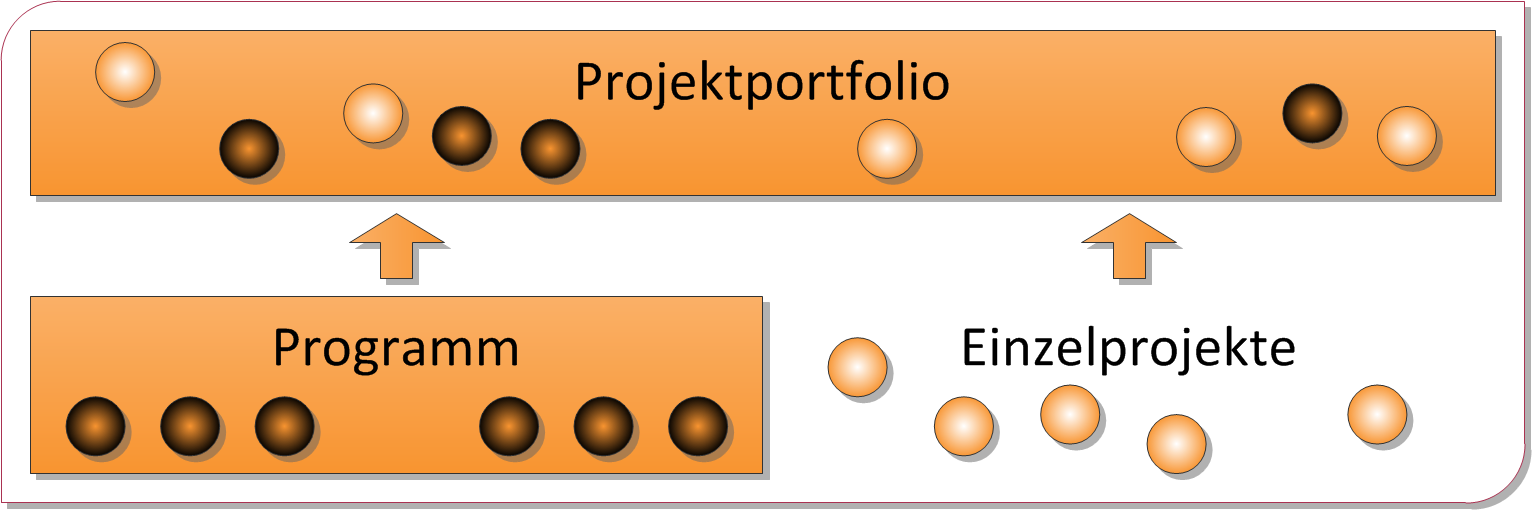
\includegraphics[width=0.8\textwidth]{Images/projektportfolio.png}
%\label{abb5}
%
%   {\footnotesize In Anlehnung an: \cite{Foschiani1999}, S.21--22]}
%   \caption[Zusammenhang von Einzelprojekten, Programm und Projektportfolio]{Zusammenhang von Einzelprojekten, Programm und Projektportfolio}
%\end{center}
%
%
%
%
%\end{figure}
%%\end{floatingfigure}
%
%\subsection{Strategische Projektplanung}
%\label{sec:SPP}
%Grundlage der strategischen Projektplanung sind die Unternehmensziele, die wesentliche Auswahlkriterien für die Projekte liefern. Die Projekte müssen mit den strategischen Zielen harmonieren. Ein Unternehmen mit dem strategischen Ziel schnelles Wachstum durch Ausweitung des Marktanteils wird Projekte anders beurteilen als ein Unternehmen, das die Gewinnmaximierung durch Kostensenkung verfolgt.
%Aufgrund der hohen Projektanzahl im Projektportfolio des strategisches Projektmanagements konkurrieren unterschiedliche Projekte um zumeist knappe Unternehmensressourcen\footnote{Vgl. \cite{Kunz2007}, S.~1}. Die Projektwünsche erreichen das Portfolio entweder Top-Down durch die Unternehmensleitung oder Bottom-Up durch die Fachbereiche. Dabei ist sicherzustellen, dass Projektideen nicht von vornherein abgeblockt oder bevorzugt werden. Jeder Vorschlag sollte zunächst die gleiche Chance haben. Ansonsten besteht die Gefahr, dass sinnvolle Vorhaben nicht realisiert werden\footnote{Vgl. \cite{Fiedler2008}, S~36}.
%Zu Beginn der Projektportfolioplanung ist eine Gesamtbetrachtung aller Projekte anzustreben. Deswegen sollte man auch die bereits genehmigten und die laufenden Projekte in die Analyse einbeziehen. Es kann durchaus sein, dass schon genehmigte Vorhaben aufgrund der nachfolgenden Bewertung verschoben oder nicht realisiert werden\footnote{Vgl. \cite{Fiedler2008}, S.~39}.
%\begin{figure}[htbp]
%%\begin{floatingfigure}[htbpr]{0.43\textwidth} 
%\begin{center}
%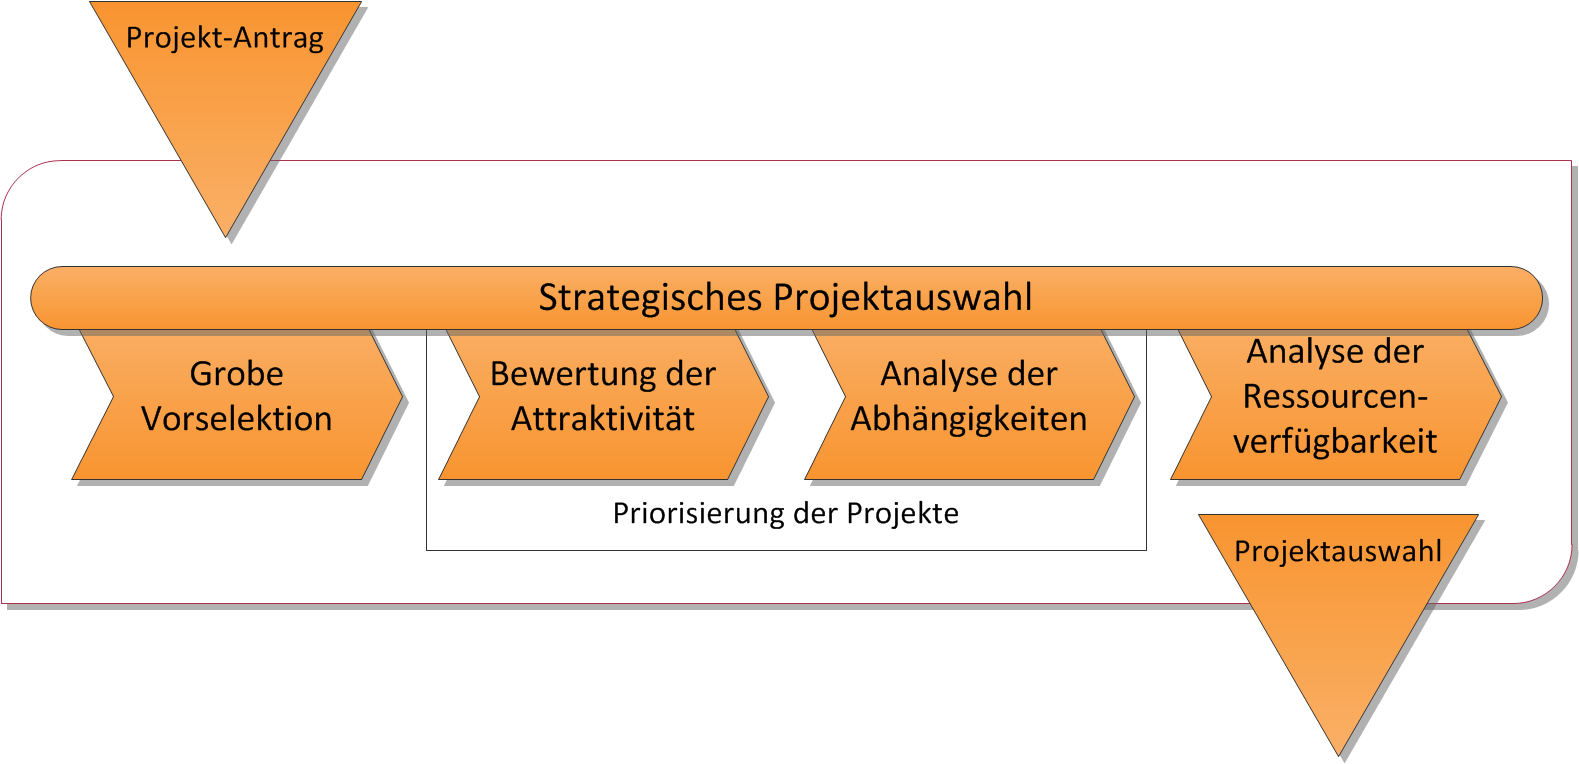
\includegraphics[width=0.8\textwidth]{Images/prozessProjektauswahl.png}
%\label{abb6}
%
%   {\footnotesize In Anlehnung an: \cite{Archer1999}, S. 208}
%   \caption[Prozess der strategischen Projektauswahl]{Prozess der strategischen Projektauswahl}
%\end{center}
%
%\end{figure}
%%\end{floatingfigure}
%In der Abbildung \ref{abb6} auf Seite \pageref{abb6} wird der Prozess der strategischen Projektauswahl dargestellt. Die strategische Projektplanung nutzt diesen Ablauf, um die vorgeschlagenen Projekte im Einklang mit der Unternehmensstrategie auf die wirklich wichtigen zu beschränken. Die hierbei zum Einsatz kommenden Methoden liefern einheitliche Beurteilungskriterien und reduzieren die Gefahr, knappe Ressourcen zu verschwenden. Die strategische Projektplanung liefert so eine  Entscheidungsfundierung, auf Basis derer das Management die letztendliche Projektauswahl trifft\footnote{Vgl. \cite{Fiedler2008}, S.~85}.
%
%Die grobe Vorselektion prüft neben der Machbarkeit, ob die Projektvorschläge den strategischen Zielen offensichtlich widersprechen. In dieser Phase kann es zur Definition von Muss-Projekten kommen. Dabei handelt es sich um Vorhaben, die z. B. aufgrund gesetzlicher Vorschriften unumgänglich sind\footnote{Vgl. \cite{Fiedler2008}, S.~41}.
%
%Im Schritt Bewertung der Attraktivität wird die Attraktivität der Projekte für das unternehmen detailliert bewertet. Die wichtigsten Bewertungskriterien sind:
%\begin{compactitem}
%\item Strategische Bedeutung (Wettbewerbsvorteile, Kundenorientierung),
%\item Dringlichkeit,
%\item Wirtschaftlichkeit,
%\item Risiko,
%\item Kosten (Entwicklungskosten, Folgekosten),
%\item Ressourcenbedarf\footnote{Vgl. \cite{Fiedler2008}, S.~41}.
%\end{compactitem}
%Rudolf Fiedler schreibt über die Aufgabe des Projektcontrollings bei der Bewertung der Attraktivität:
%\begin{quote}
%Das Projektcontrolling hat die Aufgabe, Hilfestellung beim Einsatz von Bewertungsinstrumenten zu geben und die Konsistenz der zur Beurteilung herangezogenen Daten zu prüfen.\footnote{\cite{Fiedler2008}, S. 42}
%\end{quote}
%Für eine Gesamtbetrachtung aller Einflussfaktoren der Projektbewertung bietet sich die Nutzwertanalyse an. Weitere Instrumente zur Bestimmung der Attraktivität sind auch Portfolios und Wirtschaftlichkeitsrechnungen. Ein weiterer wichtiger Bestandteil ist die Risikoanalyse, um das Erfolgspotenzial der Projekte abzuschätzen\footnote{Vgl. \cite{Fiedler2008}, S. 42}.
%[s. Kommentar] %zu wenig? dann noch Bilder von Nutzwert, Risiko, Portfolios und Wirtschaftlichkeitsanalysen einfügen.
%
%In der Analyse der Abhängigkeiten werden die gegenseitigen Einflüsse der Portfolioprojekte untersucht. Ein Projekt kann bereits in der Konzeptionsphase anderer Projekte zur veränderten Vorraussetzungen führen. Auch müssen manche Projekte mit anderen zusammen realisiert werden, da nur so das Gesamtziel erreicht werden kann. Gerade wenn verschiedene Projekte aufeinander aufbauen, hat dies ggf. signifikante Auswirkungen auf die Kosten der Umsetzungen.
%Die Ergebnisse der Auswirkungen stehen also in einem kausalen Zusammenhang mit der Attraktivität und bestimmen gleichermaßen die Priorität der Vorhaben\footnote{Vgl. \cite{Fiedler2008}, S. 79}. 
%
%Nachdem die Projekte vorselektiert, detailliert analysiert und priorisiert wurden, wartet die \glqq Hitliste\grqq der effektivsten Projekte aus die Zuteilung der meist knappen finanziellen Mittel und qualifizierten Ressourcen. Die Analyse der Ressourcenverfügbarkeit ordnet die erforderlichen Ressourcen nach Qualifikationsprofilen und die finanziellen Mittel nach den Budgets Projektklassen zu. Budgets für unterschiedliche Projektklassen werden gebildet, da gerade IT-Projekte oft große Teile des zur Verfügung stehenden Budgets aufzehren und so keine Mittel mehr für andere Projektarten zur verwendet werden können.
%Ergebnis dieser Untersuchung kann auch sein, dass Projektstarts verschoben, Leistungsumfänge gekürzt oder gar laufende Projekte gestoppt werden\footnote{Vgl. \cite{Fiedler2008}, S.~81--82}.
%
%\subsection{Strategische Projektkontrolle}
%\begin{figure}[htbp]
%%\begin{floatingfigure}[htbpr]{0.43\textwidth} 
%\begin{center}
%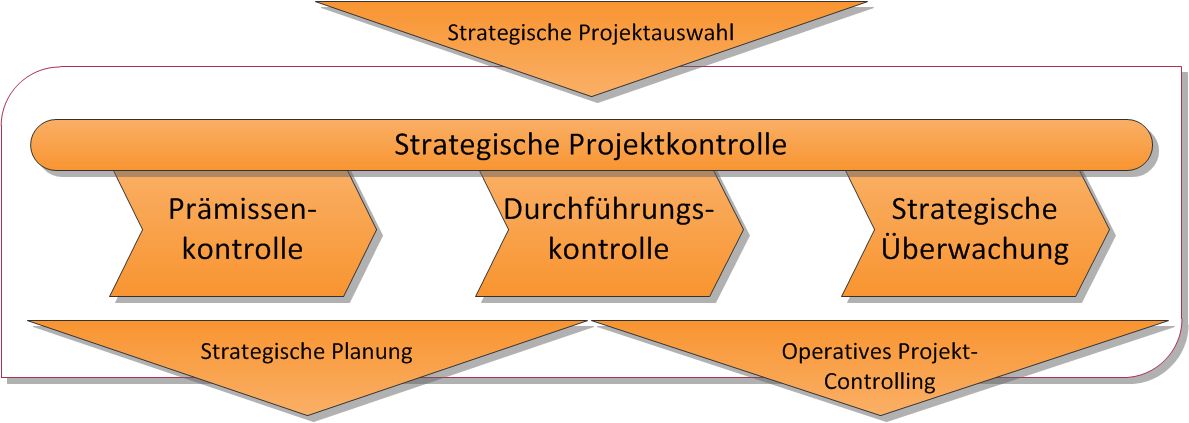
\includegraphics[width=0.8\textwidth]{Images/prozessStratKontrolle.png}
%   %{\footnotesize In Anlehnung an: \cite{Steinmann&Schreyogg2000}, S. 221}
%   \caption[Prozess der strategischen Projektkontrolle]{Prozess der strategischen Projektkontrolle}\label{abb6}
%\end{center}
%
%\end{figure}
%%\end{floatingfigure}
%Die strategische Projektkontrolle unterteilt sich in die drei wichtige Aufgaben\footnote{Vgl. \cite{Steinmann&Schreyogg2000}, S. 221}:
%\begin{compactitem}
%\item Prämissenkontrolle,
%\item Durchführungskontrolle und
%\item strategische Überwachung.
%\end{compactitem}
%Die Prämissenkontrolle untersucht während Projektauswahl und Projektdurchführung das gesamte Projektportfolio auf seine Ausgewogenheit und Stimmigkeit im Bezug auf die strategische Ausrichtung des Unternehmens. Sie stellt sicher, dass die in den Projektportfolios enthaltenen Projekte weiterhin den aktuellen strategischen Prämissen entsprechen. Hierzu sind gegebenenfalls einzelnen Projekte neu zu priorisieren\footnote{Vgl. \cite{Kunz2007}, S.~37}. 
%
%Im Rahmen der Durchführungskontrolle werden Informationen von allen Portfolioprojekten generiert, um den Fortschritt der einzelnen Projekte zu verfolgen. Mittels Definition messbarer Meilensteine, deren Ist-Ergebnisse mit der ursprünglichen Zielsetzung verglichen werden, werden strategisch relevante Problemfälle innerhalb des Projektportfolios identifiziert. Bei signifikanten Abweichungen sind Gegenmaßnahmen einzuleiten\footnote{Vgl. \cite{Kunz2007}, S.~37}~\footnote{Vgl. \cite{Fiedler2008}, S.~87}. Geeigneter Methoden der Durchführungskontrolle sind z. B. Variationen der Balanced Scorecard (Projekt--Scorecard), Checklisten oder Portfiliotechniken (Mapping Grids).
%
%Neben diesen Kontrollaktivitäten, die vor allem auf die Sicherstellung der zielgerichteten Durchführung von Projekten abzielen, fungiert die strategische Überwachung als ungerichtete flächendeckende Kontrolle als Ergänzung der beiden erstgenannten Kontrollen\footnote{Vgl. \cite{Fiedler2008}, S.~89}. Durch die Zusammenführung von Ergebniskontrolle und während der Projektdurchführung mitlaufender Wissensgenerierung werden die Projekte regelmäßig auf ihre Zielerreichung im Kontext der Unternehmensstrategien hin untersucht\footnote{Vgl. \cite{Kunz2007}, S.~37}.
%%\subsection{Projekt-Scorecard}

\section{One.Finance der Deutschen Telekom AG}
\subsection{Das Programm One.ERP}
\abk{DTAG}{Deutsche Telekom AG}
One.ERP ist eine strategische Initiative der DTAG (Deutsche Telekom AG), die die Vereinheitlichung der Datenmodelle und Prozesse auf Basis von SAP zum Ziel hat. Der Auftrag des Programms ist die Standardisierung der Daten, Prozesse und der IT-Landschaft in den Bereichen Finanzen, Human Resources, Einkauf und Logistik. Mit One.ERP wird ein lückenloses und überschneidungsfreies System entstehen, das für den Konzern weltweit einsetzbar ist. Die Vision: In Zukunft haben wir gleiche IT- und Datenstrukturen, gleiche Erfassungsprozesse und verwenden beim gleichen Vorgang den gleichen Beleg. Damit reduziert One.ERP die Komplexität und die Kosten für den Unterhalt der IT-Landschaft. Das Rechnungswesen (FI, CO) wird zukünftig in einem zentralen SAP ERP Financials System abgebildet, welches vom Programm One.ERP den Namen One.Finance erhalten hat. \\
Sechs Fachprojekte, 16 Länder\footnote{Deutschland, Albanien, Bulgarien, Griechenland, Großbritannien, Kroatien, Mazedonien, Montenegro, Niederlande, Österreich, Polen, Rumänien, Slowakei, Tschechien, Ungarn und die USA} und rund 1.000 Mitarbeiter des Konzerns arbeiten weltweit gemeinsam an der Umsetzung des Programms One.ERP.

\subsection{Standardisiertes Datenmodell}
In der komplexen Systemlandschaft der Telekom waren bisher die unterschiedlichsten Systeme im Einsatz, die auf jeweils eigenen Datenmodellen basierten. 
In dieser gewachsenen heterogenen Infrastruktur mussten die Schnittstellen so aufgebaut sein, dass trotz unterschiedlicher Datenmodelle eine Kommunikation zwischen den Systemen ermöglicht wurde. Die Pflege dieser individuell eingerichteten Schnittstellen erzeugte neben dem hohen Verwaltungsaufwand auch sehr hohe Kosten.
Im Rahmen der Standardisierung und Vereinheitlichung durch das Programm One.ERP wird diese komplexe System- und Prozesslandschaft sukzessive auf eine Plattform bestehend aus einer geringen Anzahl an Standardsystemen reduziert. Diese Systeme basieren auf dem gleichen Datenmodell, wodurch die Einrichtung von Schnittstellen vereinfacht wird und redundanter Pflegeaufwand entfällt.
Um die bestehenden Prozesse in der neuen Plattform abbilden zu können, wurden die bestehenden Datenmodelle, sowie deren Entsprechung in den anderen Systemen, erfasst und in das neue standardisierte Datenmodell mit folgendem Umfang überführt.
\begin{compactitem}    
\item    Einkauf (Procurement)
\item    Finance (Finanzen \& Controlling)
\item    HWL (Handelswaren Logistik)
\item    HR (Human Resources)
\item    IT (Allgemeine Einstellungen)
\item    PSL (Produktion Service \& Logistik)
\end{compactitem}

\subsection{Zukünftige Konzernstruktur (One.Finance)}
tbd
\subsection{Reporting - Data Hub (One.Finance)}
Das Reporting-Gesamtkonzept sieht vor, dass die verschiedenen Informationsbedarfe der Berichtsempfänger durch unterschiedliche Berichtsprodukte bedient werden sollen. 
Der Data Hub, ein SAP BW System\abk{SAP BW}{SAP Business Warehouse - Business Intelligence Lösung der SAP} (Business Intelligence Lösung der SAP), ist hierbei die zentrale Schnittstelle. Im Data Hub erfolgt die technische Bereitstellung von Daten aus dem transaktionalen System für bereichsspezifische Berichte von nachgelagerten Funktionen.
Die Standardberichte in One.ERP basieren auf einem konzernweit vereinheitlichten Kontenplan, um ein gemeinsames Verständnis der dargestellten Ergebnisse zu fördern -- getreu dem Credo „Eine Zahl -- eine Wahrheit“. Alle Berichte sind damit so aufgebaut, dass konzernweit anwendbare Anforderungen an die externe oder interne Berichterstattung berücksichtigt sind und ein möglichst einfaches Arbeiten mit den Berichten ermöglicht wird. 
Bei den Standardberichten handelt es sich in der Regel um eigenentwickelte Berichte, die mittels SAP-Standard-Reportingtools realisiert werden. Diese maßgeschneiderten Nicht-SAP-Standardberichte erfüllen eine hohe Prozesseffizienz und Datenqualität, um die Informationsanforderungen möglichst effektiv und effizient zu erfüllen.
\subsubsection{Externe Standardberichte}
Die externen Standardberichte sind die Basis für die externe Berichterstattung aller Gesellschaften des Konzerns Deutsche Telekom für den Einzelabschluss und ebenso für die Konzernberichterstattung. Die Berichte sind darüber hinaus auch die Grundlage für die Prüfung der Gesellschaft durch Wirtschaftsprüfer. 
Weiterhin gibt es eine Kontrollfunktion durch die externen Standardberichte. Die Zahlen, die hier dargestellt werden, ermöglichen eine laufende Überprüfung der Liquidität und Wirtschaftlichkeit und erlauben es, konkrete Handlungsempfehlungen für einzelne Abteilungen zu erarbeiten und dem Management als Entscheidungsgrundlage zu dienen. Zur Erstellung dieser Standardberichte wird hierbei vollständig auf One.Finance und das neue Hauptbuch zurückgegriffen. \abk{One.Finance}{SAP ERP Financials im Programm One.ERP}\\
Externe Standardberichte im One.ERP Data Hub:
\begin{compactitem}  
\item 	  Bilanz
\item     Gewinn- und Verlustrechnung (Gesamtkostenverfahren)
\item     Gewinn- und Verlustrechnung (Umsatzkostenverfahren)
\item     Anlagenspiegel
\item    Rückstellungsspiegel
 \item    Eigenkapitalsveränderungsrechnung
\item     Gesamtergebnisrechnung
 \item    Kapitalflussrechnung (ohne Umgliederungen)
\end{compactitem}
\subsubsection{Interne Standardberichte}
Die internen Standardberichte dienen der Analyse der Wirtschaftlichkeit und Effizienz sowie als Basis für die interne Steuerung. Neben den klassischen Kostenstellen-, Kostenträger- und Profit Center Berichten zählen auch die Berichte der wertschöpfungsorientierten Steuerung, das Konzernergebnisschema (GPS) sowie die Functional P\&L zu den internen Standardberichten, die insbesondere für die Controlling-Bereiche der Deutschen Telekom ein wesentliches Hilfsmittel darstellen. Zur Erstellung dieser Standardberichte wird hierbei auf die Module FI und CO in One.Finance zurückgegriffen.\\
Interne Standardberichte im One.ERP Data Hub:
\begin{compactitem}  
\item 		Bilanz
\item     Kostenstellenbericht
\item     Kostenträgerbericht
\item     Profit Center Bericht
\item     Group Performance Statement (Konzernergebnisschema)
\item     Operating Free Cash Flow
\item     Operating Working Capital
\item    Functional Profit and Loss Statement (FP\&L)
\end{compactitem}
\section{Fazit}
ERP-Software für das Finanzmanagement optimiert Abläufe des betrieblichen Rechnungswesen. Die SAP ERP-Anwendungen FI und CO können mit allen anderen Komponenten der Wertschöpfungskette integriert werden. Sie sparen Kosten und Zeit durch die Automatisierung von Geschäftsprozessen und schaffen im Rechnungswesen mehr Vertrauen durch eine zuverlässige Kontrolle finanzieller Risiken. 

Die SAP ERP Financials Module FI und CO sind elementare Bestandteile der Betriebswirtschaft und in jedem Unternehmen einsetzbar. Andere  Standard- oder eigenerstellte Softwarelösungen haben in deutschen Großunternehmen fast keine Bedeutung mehr\footnote{Vgl. \cite{Gleich2010}, S. 58}. Sie erfüllen sowohl die Vorgaben der gesetzlich vorgeschriebenen externen Rechnungslegung, als auch die vielfältigen Anforderungen an interne Analysen und Reportings im internen Rechnungswesen. 

Das Konzernprogramm One.ERP der Deutschen Telekom AG setzt ein Prozess-Tool um, das flexibel, schnell, standardisiert und kosteneffizient ist. Dies hat den wesentlichen Vorteil, dass unabhängig vom Buchungskreis ein Geschäftsvorfall immer den gleichen Buchungsprozess bedingt. Für die Tochter Telekom Deutschland GmbH etwa bedeutet dies, dass die IT-Systeme von drei ehemals \glqq unabhängigen\grqq \ Gesellschaften (T-Home, T-Mobile, Geschäftskunden) zukünftig einheitlich abgebildet werden. Es muss nur noch ein System gepflegt werden, Rollouts werden nur noch einmal erforderlich sein und die IT-Kosten werden gesenkt. Bei zukünftigen Organisationsänderungen entfallen vielfältige Abstimmungsrunden, da es nur den einen Prozess gibt. Für alle Legaleinheiten des Konzerns, wird gerade durch die einheitliche Implementierung des Rechnungswesens in SAP ERP Financials, ein single point of truth geschaffen, welcher eine erstmals einheitliche Basis für die Geschäftssteuerung liefert.

Um langfristig im internationalen Wettbewerb bestehen zu können, sind im Zwang permanenter Veränderungen, agile und flexible Reaktionen unumgänglich. One.ERP ist für die Zukunft der Deutsche Telekom AG alternativlos.
\newpage
\section{Anhang}
\subsection{Anhang 1}
\label{sec:Anhang1}
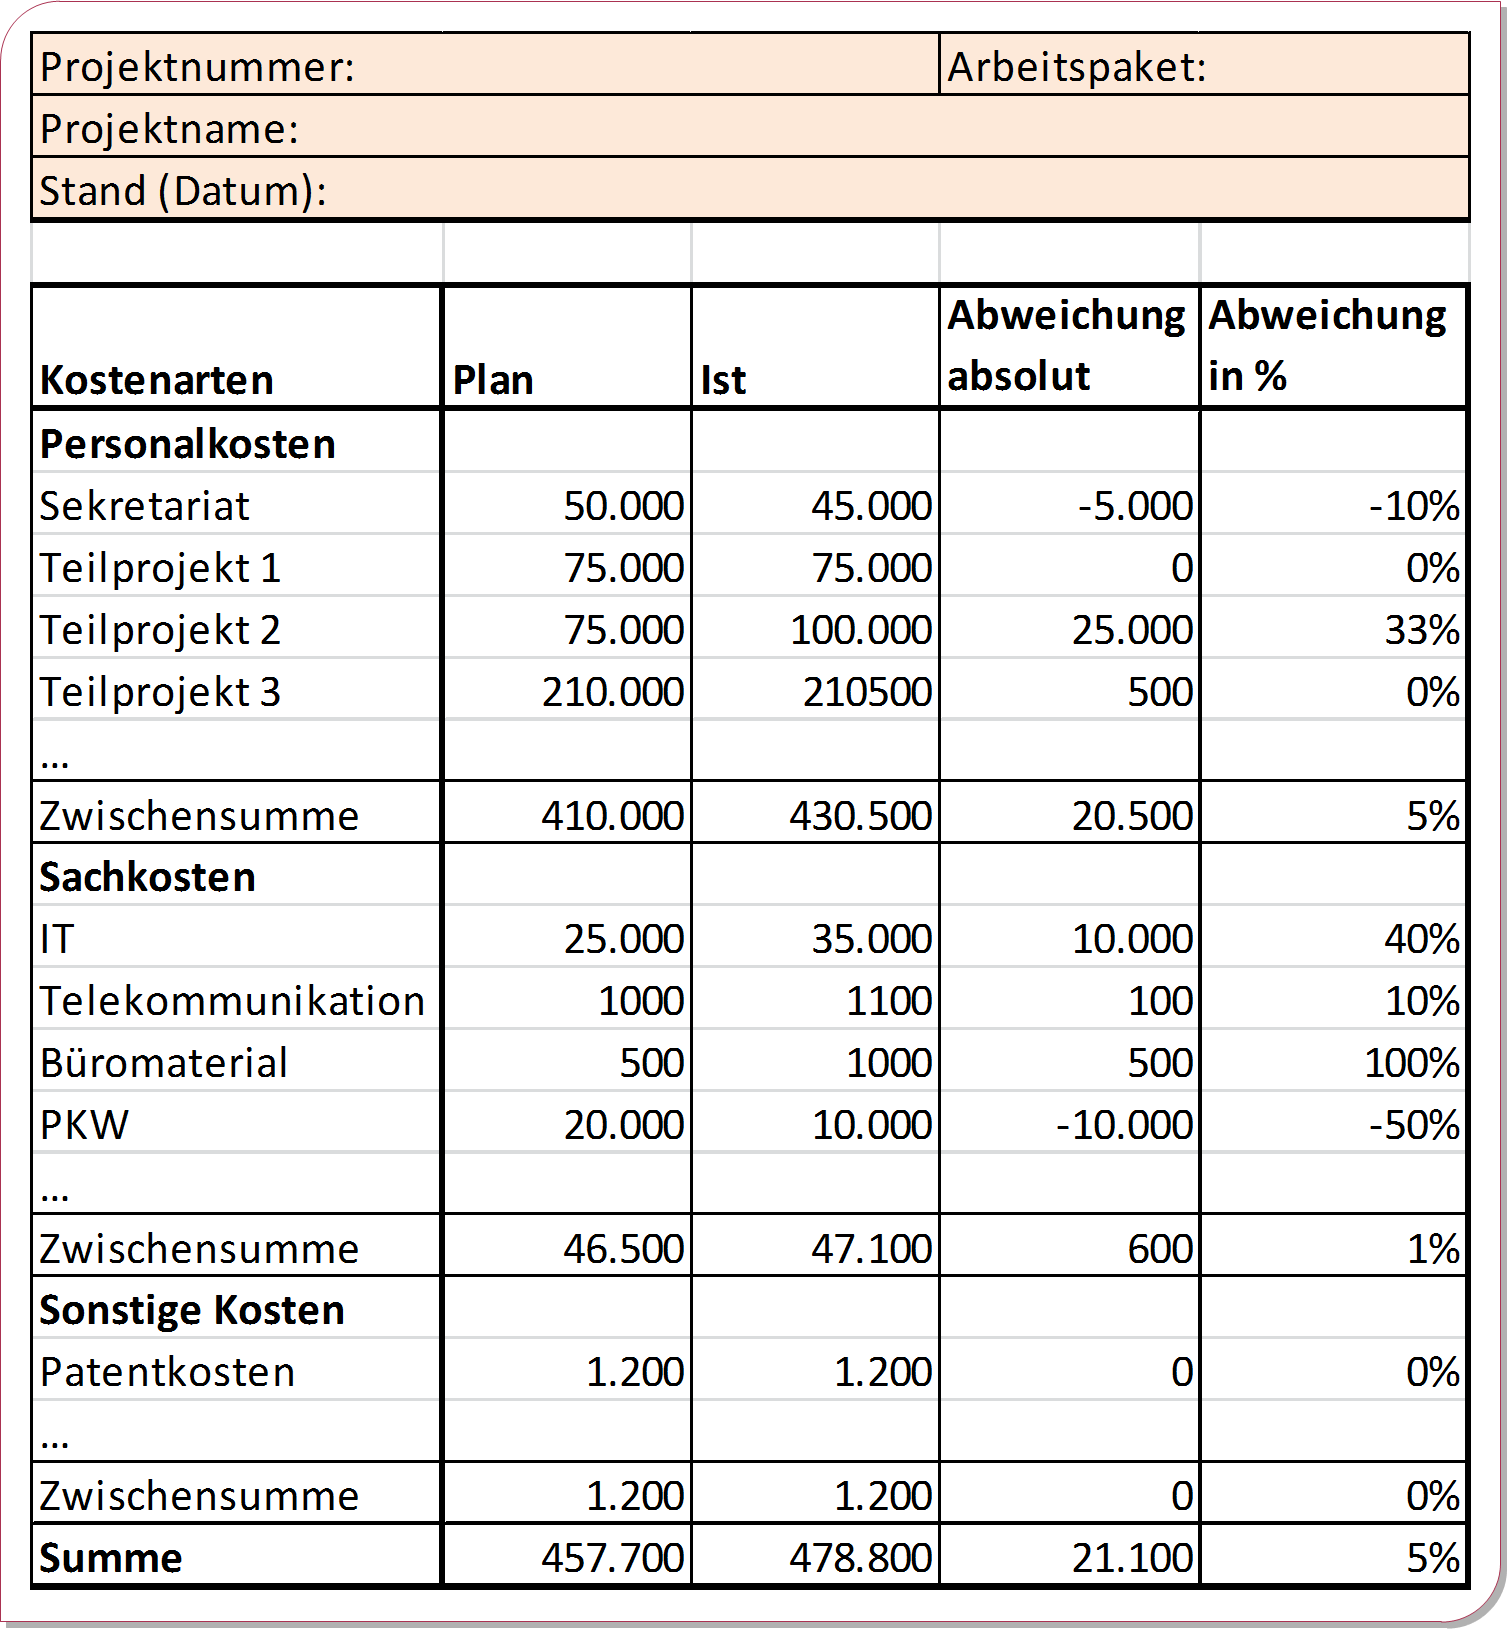
\includegraphics[width=1\textwidth]{Images/PlanIstVergleich.png} 
\begin{center}
   {\footnotesize In Anlehnung an: \cite{Blazek2001}, S. 137}\\
   Einfacher Plan-Ist-Vergleich
   %   \caption[Einfacher Plan-Ist-Vergleich]{Einfacher Plan-Ist-Vergleich}\label{abb3}
\end{center}
%\end{figure}
%\end{floatingfigure}
\newpage
\subsection{Anhang 2}
\label{sec:Anhang2}
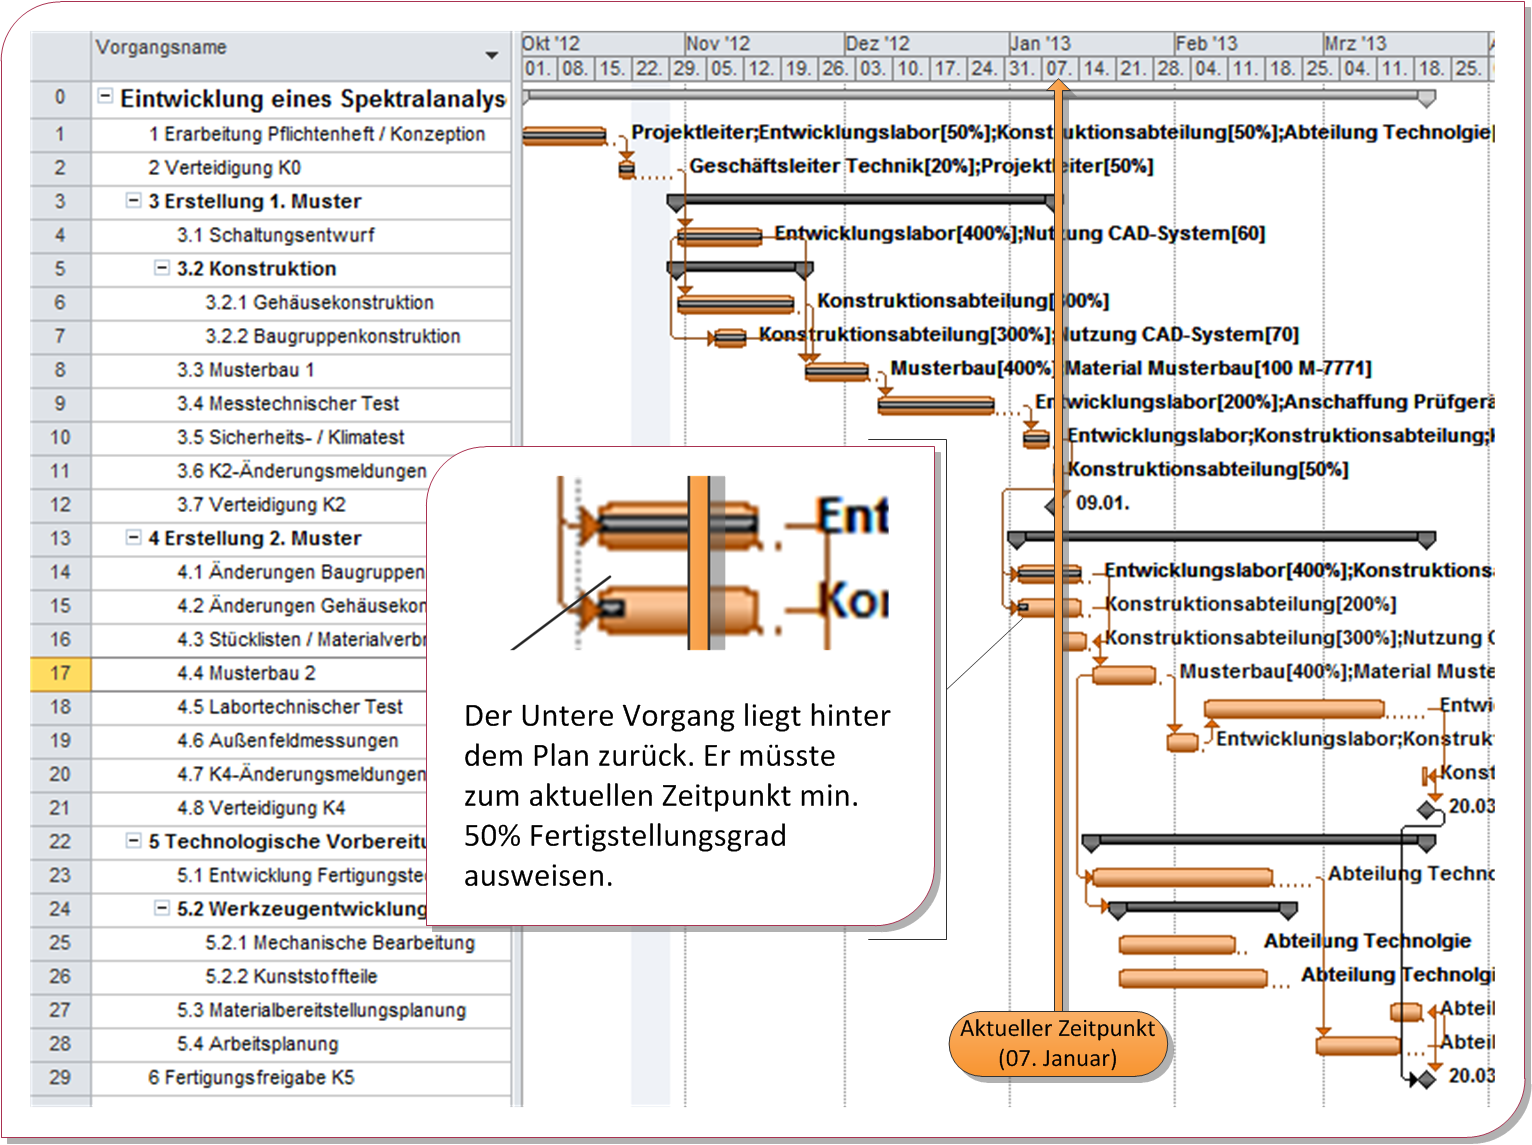
\includegraphics[width=1\textwidth]{Images/MSPfortschritt.png} 
\begin{center}
   %{\footnotesize In Anlehnung an: \cite{Blazek2001}, S. 137}\\
   Projektfortschrittsbericht in MS-Project
   %   \caption[Einfacher Plan-Ist-Vergleich]{Einfacher Plan-Ist-Vergleich}\label{abb3}
\end{center}
%\end{figure}
%\end{floatingfigure}
\newpage

\newpage
%%Abkürzungsverzeichnis z.B. etc.\abk{etc.}{et cetera}
 \section{Fachwort- und Abkürzungsverzeichnis}
\printnomenclature
\newpage

%tabellenverzeichnis
\section{Abbildungsverzeichnis}
%\addsec{Abbildungsverzeichnis}
\renewcommand{\listfigurename}{} 
\listoffigures
\newpage

%abbildungsverzeichnis
\section{Tabellenverzeichnis}
\renewcommand{\listtablename}{} 
\listoftables
\newpage

%Literaturverzeichnis
\renewcommand\refname{Literatur- und Quellenverzeichnis}
\nocite{*}
\bibliographystyle{agsm}
\bibliography{includes/quellen}
\newpage

%ehrenwoertliche erklaerung
\thispagestyle{empty}
\clearpage

\section*{Ehrenwörtliche Erklärung}
Hiermit versichere ich, dass die vorliegende Arbeit von mir selbstständig und 
ohne unerlaubte Hilfe angefertigt worden ist, insbesondere dass ich alle Stellen, die wörtlich oder annähernd wörtlich aus Veröffentlichungen entnommen sind, durch Zitate als solche gekennzeichnet habe. Ich versichere auch, dass die von mir eingereichte schriftliche Version mit der digitalen Version übereinstimmt. 
Weiterhin erkläre ich, dass die Arbeit in gleicher oder ähnlicher Form noch keiner anderen Prüfungsbehörde vorgelegen hat. Ich erkläre mich damit einverstanden/nicht einverstanden, dass die Arbeit der Öffentlichkeit zugänglich gemacht wird. Ich erkläre mich damit einverstanden, dass die Digitalversion dieser Arbeit zwecks Plagiatsprüfung auf die Server externer Anbieter hoch geladen werden darf. Die Plagiatsprüfung stellt keine Zurverfügungstellung für die Öffentlichkeit dar.\section*{Declaration in lieu of oath}
I hereby declare that I produced the submitted paper with no assistance from any other party and without the use of any unauthorized aids and, in particular, that I have marked as quotations all passages, which are reproduced verbatim or nearby-verbatim from publications. Also, I declare that the submitted print version of this thesis is identical with  its digital version. Further, I declare that this thesis has never been submitted before to any other examination board in either its present form or in any other similar version. I herewith agree/disagree that this thesis may be published. 
I herewith consent that this thesis may be uploaded to the server of external contractors for the purpose of submitting it to the contractors’ plagiarism detection systems. Uploading this thesis for the purpose of submitting it to plagiarism detection systems is not a form of publication.\\[0.5cm]
René Spieker:\\[1cm]
\line(1,0){100} \hfill \line(1,0){150}\\
(Ort, Datum) \hfill (Eigenhändige Unterschrift)\\[1cm]
Tobias Wäschle:\\[1cm]
\line(1,0){100} \hfill \line(1,0){150}\\
(Ort, Datum) \hfill (Eigenhändige Unterschrift)








\lfoot{\LaTeX}
\end{document}